\documentclass{beamer}
\usetheme{Madrid}
\usepackage[T1]{fontenc}
\usepackage{mathpazo}
\usepackage{graphicx}
\usepackage{booktabs}
\usepackage{tikz}
\usetikzlibrary{positioning,arrows.meta,shapes.geometric,fit,backgrounds,calc}
\definecolor{cetnavy}{RGB}{10,26,63}
\definecolor{cetlight}{RGB}{225,231,242}
\setbeamercolor{structure}{fg=cetnavy}
\setbeamercolor{frametitle}{bg=cetnavy,fg=white}
\setbeamercolor{title}{bg=cetnavy,fg=white}
\setbeamertemplate{navigation symbols}{}
% =====================================================================
%  EDIT YOUR DETAILS HERE — this ONE file feeds every abstract & deck.
%  (Change a value, recompile; all 36 documents update.)
% =====================================================================
\newcommand{\seminarName}{Aflah Muhammed P}      % <-- your full name (guessed from your email; please verify)
\newcommand{\seminarRoll}{TVE00CS000}            % <-- your university register/roll number
\newcommand{\seminarClassRoll}{00}               % <-- your class roll no (the short one)
\newcommand{\seminarGuide}{Prof.\ <Guide Name>}  % <-- your guide
\newcommand{\seminarDept}{Department of Computer Science and Engineering}
\newcommand{\seminarCollege}{College of Engineering Trivandrum}
\newcommand{\seminarShortCollege}{CET}           % shown in the slide footer, e.g. "Aflah Muhammed P (CET)"
\newcommand{\seminarShortTitle}{B.Tech Seminar}  % middle of the slide footer
\newcommand{\seminarDate}{July 31, 2026}
% ---------------------------------------------------------------------
% Optional: put a logo image named  cet_logo.png  in this folder and it
% will appear on every title slide automatically. If absent, it is skipped.
% =====================================================================

\title[\seminarShortTitle]{A Survey on the Evaluation of LLM-based Agents}
\author[\seminarName\ (\seminarShortCollege)]{\seminarName \\ \seminarRoll \\ Roll No: \seminarClassRoll \\ Guide: \seminarGuide}
\institute[\seminarShortCollege]{\seminarDept \\ \seminarCollege}
\date{\seminarDate}
\titlegraphic{\IfFileExists{cet_logo.png}{\includegraphics[height=1.1cm]{cet_logo.png}}{}}
\begin{document}
\begin{frame}\titlepage\end{frame}
\begin{frame}{Table of Contents}\tableofcontents\end{frame}
\section{Introduction}
\begin{frame}{Introduction}
\textbf{\textit{From single-shot LLMs to autonomous agents}}
\begin{itemize}
\item LLM-based agents plan, use tools, and act.
\item They operate over long, multi-step trajectories.
\item Deployed in web, coding, and science tasks.
\item Evaluation lags behind rapid agent progress.
\end{itemize}
\end{frame}
\begin{frame}{Introduction}
\textbf{\textit{Why a survey on evaluation?}}
\begin{itemize}
\item Benchmarks are fragmented across many domains.
\item No shared map of what to measure.
\item This paper organizes the evaluation landscape.
\item Guides practitioners toward meaningful assessment.
\end{itemize}
\end{frame}

\section{Literature Survey}
\begin{frame}{Literature Survey}
\textbf{\textit{Prior evaluation efforts}}
\begin{itemize}
\item Static NLP benchmarks measure single outputs only.
\item Agent benchmarks: AgentBench, GAIA test broad tasks.
\item Capability studies isolate planning and tool use.
\item Framework tools (LangSmith, Langfuse) trace runs.
\item Prior surveys cover agents, not their evaluation.
\end{itemize}
\end{frame}

\section{Motivation}
\begin{frame}{Motivation}
\textbf{\textit{Evaluation is the bottleneck}}
\begin{itemize}
\item Final-answer accuracy hides broken reasoning steps.
\item Static benchmarks saturate and become obsolete.
\item Cost, safety, and robustness rarely measured.
\item A unified taxonomy is genuinely missing.
\end{itemize}
\end{frame}

\section{Problem Statement}
\begin{frame}{Problem Statement}
\begin{itemize}
\item How are LLM-based agents currently evaluated?
\item Which capabilities and applications have benchmarks?
\item What do existing benchmarks systematically miss?
\item How should evaluation evolve with agent ability?
\end{itemize}
\end{frame}

\section{Objectives}
\begin{frame}{Objectives}
\textbf{\textit{Goals of the survey}}
\begin{itemize}
\item Map evaluation across capabilities and applications.
\item Cover generalist agents and developer frameworks.
\item Analyze core dimensions of benchmark design.
\item Identify current trends and open gaps.
\end{itemize}
\end{frame}

\section{Methodology Overview}
\begin{frame}{Methodology Overview}
\begin{center}
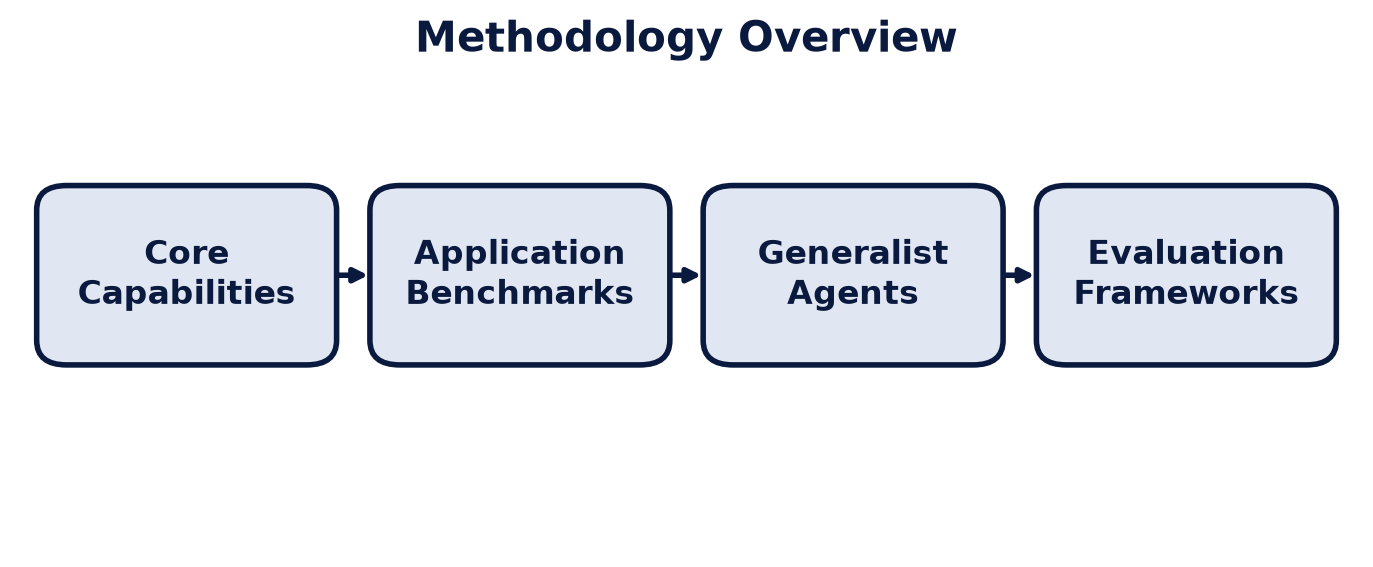
\includegraphics[width=0.9\textwidth,height=0.62\textheight,keepaspectratio]{images/evalsurvey_1.png}
\end{center}
\textbf{\textit{Four dimensions of the survey}}
\begin{itemize}
\item Skills, then domains, then holistic and tooling.
\end{itemize}
\end{frame}

\section{System Architecture}
\begin{frame}{System Architecture}
\begin{center}
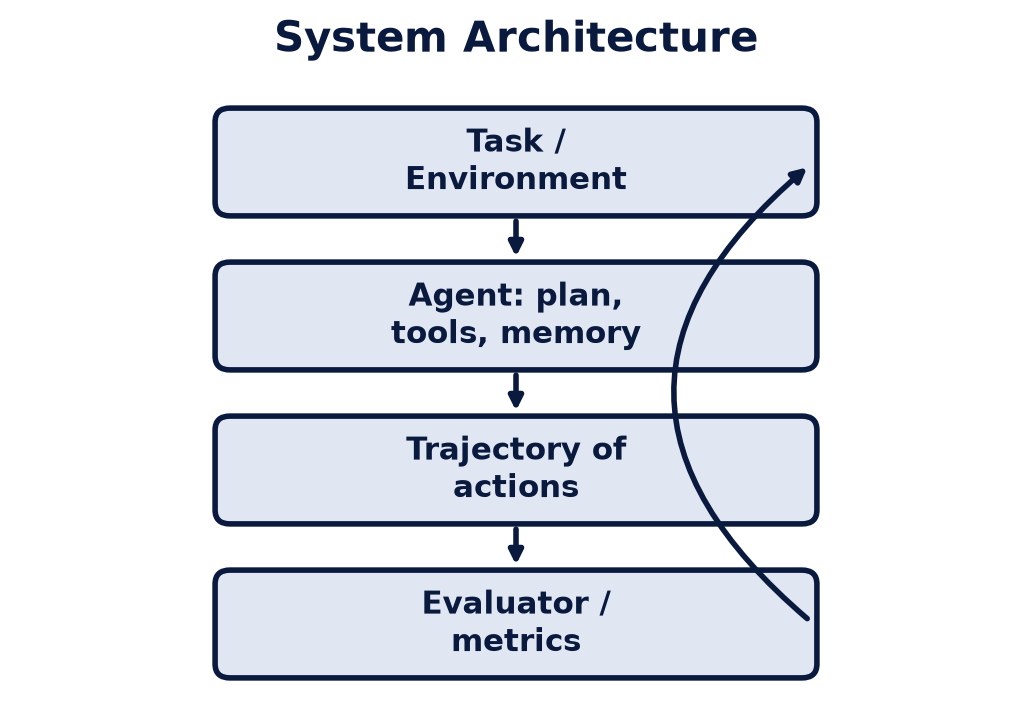
\includegraphics[width=0.9\textwidth,height=0.62\textheight,keepaspectratio]{images/evalsurvey_2.png}
\end{center}
\textbf{\textit{What an evaluation setup measures}}
\begin{itemize}
\item Both final outcome and intermediate trajectory.
\end{itemize}
\end{frame}

\section{Data Collection}
\begin{frame}{Data Collection}
\textbf{\textit{Scope and sources of the survey}}
\begin{itemize}
\item Reviews benchmarks, datasets, and framework tools.
\item Capabilities: planning, tool use, reflection, memory.
\item Domains: web, software, science, conversation.
\item Analyzes data curation, environments, and metrics.
\item Companion GitHub repo tracks the papers.
\end{itemize}
\end{frame}

\section{Model Development}
\begin{frame}{Model Development}
\begin{center}
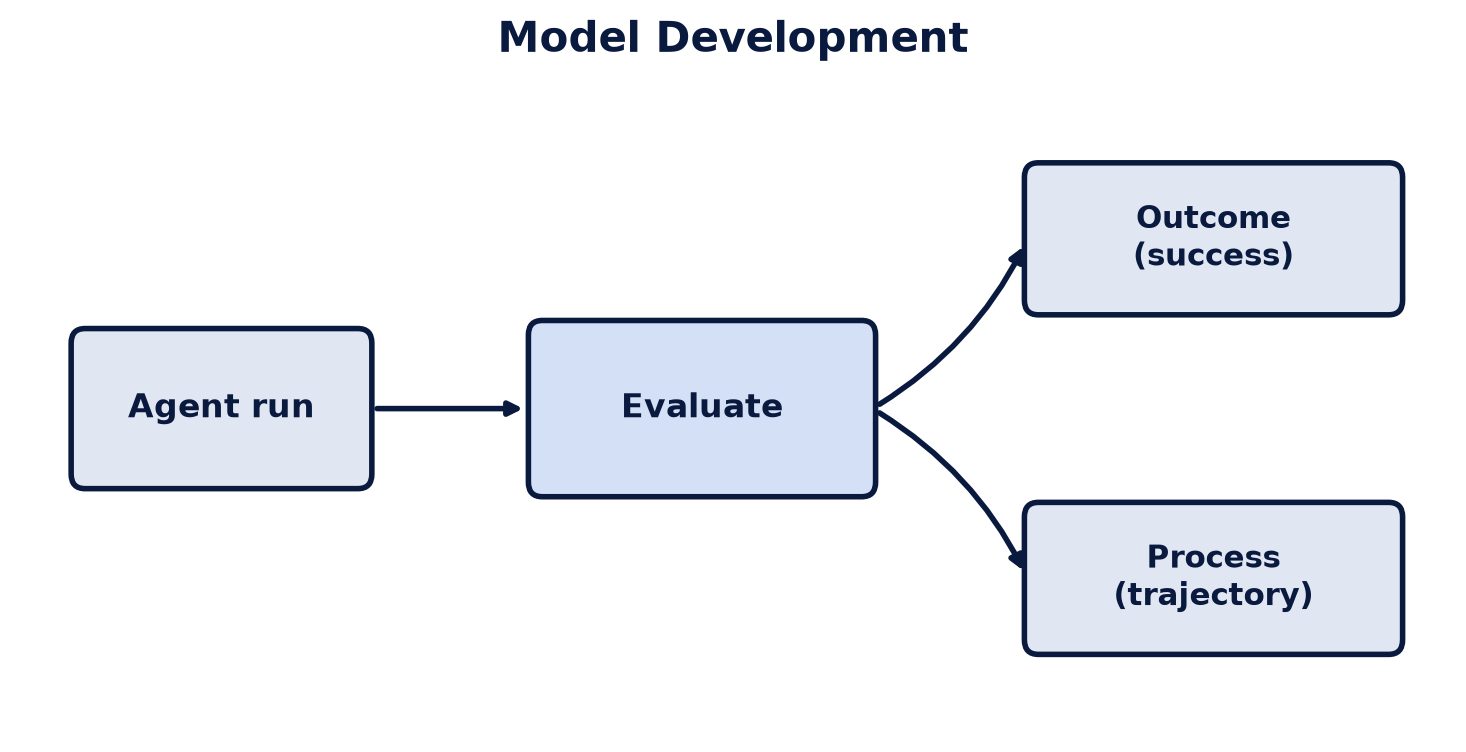
\includegraphics[width=0.9\textwidth,height=0.62\textheight,keepaspectratio]{images/evalsurvey_3.png}
\end{center}
\textbf{\textit{Two evaluation paradigms surveyed}}
\begin{itemize}
\item Coarse success vs. fine-grained step scoring.
\item Judges: rules, LLM-as-judge, agent-as-judge.
\end{itemize}
\end{frame}
\begin{frame}{Model Development}
\textbf{\textit{Representative benchmarks per capability}}
\begin{itemize}
\item Planning: PlanBench, FlowBench.
\item Tool use: BFCL, ToolLLM, ComplexFuncBench.
\item Memory: LongMemEval, MemBench, StreamBench.
\item Web: WebArena, Mind2Web, WebVoyager.
\item Software: SWE-bench and its Verified subset.
\end{itemize}
\end{frame}

\section{Results}
\begin{frame}{Results}
\textbf{\textit{Key findings across domains}}
\begin{center}
\footnotesize
\begin{tabular}{@{}ll@{}}
\toprule
\textbf{Domain} & \textbf{Example benchmarks} \\
\midrule
Web & WebArena, Mind2Web \\
Software & SWE-bench (Verified) \\
Science & ScienceAgentBench, SciCode \\
Conversation & $\tau$-bench, MultiWOZ \\
Generalist & GAIA, OSWorld, AppWorld \\
\bottomrule
\end{tabular}
\end{center}
\begin{itemize}
\item Coverage is broad but unevenly distributed.
\end{itemize}
\end{frame}
\begin{frame}{Results}
\textbf{\textit{Two dominant trends}}
\begin{itemize}
\item Shift to realistic, professional-workflow environments.
\item Rise of live, continuously-updated benchmarks.
\item Examples: SWE-bench family, iterative BFCL releases.
\end{itemize}
\end{frame}

\section{Discussions}
\begin{frame}{Discussions}
\textbf{\textit{Interpreting the landscape}}
\begin{itemize}
\item Harder benchmarks track fast-improving agents.
\item Trajectory metrics reveal why agents fail.
\item Frameworks (LangSmith, Langfuse) aid debugging.
\item Realism trades off with reproducibility.
\end{itemize}
\end{frame}

\section{Challenges}
\begin{frame}{Challenges}
\textbf{\textit{Critical gaps identified}}
\begin{itemize}
\item Cost-efficiency: tokens, latency, API expense.
\item Safety, robustness, and policy compliance.
\item Fine-grained, trajectory-level evaluation is scarce.
\item Static benchmarks saturate and leak into training.
\end{itemize}
\end{frame}

\section{Future Work}
\begin{frame}{Future Work}
\textbf{\textit{Directions the survey advocates}}
\begin{itemize}
\item Scalable, automated evaluation via LLM/agent judges.
\item Synthetic data generation for fresh tasks.
\item Standard cost and safety metrics.
\item Continuously-updated living benchmarks.
\end{itemize}
\end{frame}

\section{Conclusion}
\begin{frame}{Conclusion}
\begin{itemize}
\item First unified map of agent evaluation.
\item Spans capabilities, applications, generalists, frameworks.
\item Trend: realistic, harder, living benchmarks.
\item Gaps: cost, safety, and granular assessment.
\end{itemize}
\end{frame}

\section{References}
\begin{frame}{References}
\footnotesize
\begin{itemize}
\item A. Yehudai, L. Eden, A. Li, G. Uziel, Y. Zhao, R. Bar-Haim, A. Cohan, and M. Shmueli-Scheuer, ``Survey on Evaluation of LLM-based Agents,'' Findings of ACL, arXiv:2503.16416, 2025.
\item S. Yao et al., ``$\tau$-bench: A Benchmark for Tool-Agent-User Interaction in Real-World Domains,'' arXiv:2406.12045, 2024.
\item C. E. Jimenez et al., ``SWE-bench: Can Language Models Resolve Real-World GitHub Issues?,'' ICLR, 2024.
\item G. Mialon et al., ``GAIA: A Benchmark for General AI Assistants,'' ICLR, 2024.
\end{itemize}
\end{frame}
\begin{frame}\vfill\centering{\Huge Thank You}\vfill\end{frame}
\end{document}
